\chapter{Resultados de comandos}\label{cap1}

A codificação de todos os arquivos do \abnTeX\ é \texttt{UTF8}. É necessário que
você utilize a mesma codificação nos documentos que escrever, inclusive nos
arquivos de base bibliográficas |.bib|.

% ---
\section{Citações diretas}
\label{sec-citacao}
% ---

\index{citações!diretas}Utilize o ambiente \texttt{citacao} para incluir
citações diretas com mais de três linhas:

\begin{citacao}
As citações diretas, no texto, com mais de três linhas, devem ser
destacadas com recuo de 4 cm da margem esquerda, com letra menor que a do texto
utilizado e sem as aspas. No caso de documentos datilografados, deve-se
observar apenas o recuo \cite[5.3]{NBR10520:2002}.
\end{citacao}

Use o ambiente assim:

\begin{verbatim}
\begin{citacao}
As citações diretas, no texto, com mais de três linhas [...] deve-se observar
apenas o recuo \cite[5.3]{NBR10520:2002}.
\end{citacao}
\end{verbatim}

O ambiente \texttt{citacao} pode receber como parâmetro opcional um nome de
idioma previamente carregado nas opções da classe (\autoref{sec-hifenizacao}). Nesse
caso, o texto da citação é automaticamente escrito em itálico e a hifenização é
ajustada para o idioma selecionado na opção do ambiente. Por exemplo:

\begin{verbatim}
\begin{citacao}[english]
Text in English language in italic with correct hyphenation.
\end{citacao}
\end{verbatim}

Tem como resultado:

\begin{citacao}[english]
Text in English language in italic with correct hyphenation.
\end{citacao}

\index{citações!simples}Citações simples, com até três linhas, devem ser
incluídas com aspas. Observe que em \LaTeX as aspas iniciais são diferentes das
finais: ``Amor é fogo que arde sem se ver''.

% ---
\section{Notas de rodapé}
% ---

As notas de rodapé são detalhadas pela NBR 14724:2011 na seção 5.2.1\footnote{As
notas devem ser digitadas ou datilografadas dentro das margens, ficando
separadas do texto por um espaço simples de entre as linhas e por filete de 5
cm, a partir da margem esquerda. Devem ser alinhadas, a partir da segunda linha
da mesma nota, abaixo da primeira letra da primeira palavra, de forma a destacar
o expoente, sem espaço entre elas e com fonte menor
\citeonline[5.2.1]{NBR14724:2011}.}\footnote{Caso uma série de notas sejam
criadas sequencialmente, o \abnTeX\ instrui o \LaTeX\ para que uma vírgula seja
colocada após cada número do expoente que indica a nota de rodapé no corpo do
texto.}\footnote{Verifique se os números do expoente possuem uma vírgula para
dividi-los no corpo do texto.}. 


% ---
\section{Tabelas}
% ---

\index{tabelas}A \autoref{tab-nivinv} é um exemplo de tabela construída em
\LaTeX.

\begin{table}[htb]
\ABNTEXfontereduzida
\caption[Níveis de investigação]{Níveis de investigação.}
\label{tab-nivinv}
\begin{tabular}{p{2.6cm}|p{6.0cm}|p{2.25cm}|p{3.40cm}}
  %\hline
   \textbf{Nível de Investigação} & \textbf{Insumos}  & \textbf{Sistemas de Investigação}  & \textbf{Produtos}  \\
    \hline
    Meta-nível & Filosofia\index{filosofia} da Ciência  & Epistemologia &
    Paradigma  \\
    \hline
    Nível do objeto & Paradigmas do metanível e evidências do nível inferior &
    Ciência  & Teorias e modelos \\
    \hline
    Nível inferior & Modelos e métodos do nível do objeto e problemas do nível inferior & Prática & Solução de problemas  \\
   % \hline
\end{tabular}
\legend{Fonte: \citeonline{van86}}
\end{table}

Já a \autoref{tabela-ibge} apresenta uma tabela criada em conformidade com o padrão estabelecido pelo
\citeonline{ibge1993}, requerido pelas normas da ABNT para documentos técnicos e
acadêmicos.

\begin{table}[htb]
\IBGEtab{%
  \caption{Exemplo de tabela, conforme padrão IBGE.}%
  \label{tabela-ibge}
}{%
  \begin{tabular}{ccc}
  \toprule
   Nome & Nascimento & Documento \\
  \midrule \midrule
   Maria da Silva & 11/11/1111 & 111.111.111-11 \\
  \midrule 
   João Souza & 11/11/2111 & 211.111.111-11 \\
  \midrule 
   Laura Vicuña & 05/04/1891 & 3111.111.111-11 \\
  \bottomrule
\end{tabular}%
}{%
  \fonte{Produzido pelos autores.}%
  \nota{Esta é uma nota, que diz que os dados são baseados na
  regressão linear.}%
  \nota[Anotações]{Uma anotação adicional, que pode ser seguida de várias
  outras.}%
  }
\end{table}


% ---
\section{Figuras}
% ---

\index{figuras}Figuras podem ser criadas diretamente em \LaTeX,
como o exemplo da \autoref{fig_circulo}.

\begin{figure}[htb]
	\caption{\label{fig_circulo}A delimitação do espaço}
	\begin{center}
	    \setlength{\unitlength}{5cm}
		\begin{picture}(1,1)
		\put(0,0){\line(0,1){1}}
		\put(0,0){\line(1,0){1}}
		\put(0,0){\line(1,1){1}}
		\put(0,0){\line(1,2){.5}}
		\put(0,0){\line(1,3){.3333}}
		\put(0,0){\line(1,4){.25}}
		\put(0,0){\line(1,5){.2}}
		\put(0,0){\line(1,6){.1667}}
		\put(0,0){\line(2,1){1}}
		\put(0,0){\line(2,3){.6667}}
		\put(0,0){\line(2,5){.4}}
		\put(0,0){\line(3,1){1}}
		\put(0,0){\line(3,2){1}}
		\put(0,0){\line(3,4){.75}}
		\put(0,0){\line(3,5){.6}}
		\put(0,0){\line(4,1){1}}
		\put(0,0){\line(4,3){1}}
		\put(0,0){\line(4,5){.8}}
		\put(0,0){\line(5,1){1}}
		\put(0,0){\line(5,2){1}}
		\put(0,0){\line(5,3){1}}
		\put(0,0){\line(5,4){1}}
		\put(0,0){\line(5,6){.8333}}
		\put(0,0){\line(6,1){1}}
		\put(0,0){\line(6,5){1}}
		\end{picture}
	\end{center}
	\legend{Fonte: os autores}
\end{figure}

Ou então figuras podem ser incorporadas de arquivos externos, como é o caso da
\autoref{fig_grafico}. Se a figura que ser incluída se tratar de um diagrama, um
gráfico ou uma ilustração que você mesmo produza, priorize o uso de imagens
vetoriais no formato PDF. Com isso, o tamanho do arquivo final do trabalho será
menor, e as imagens terão uma apresentação melhor, principalmente quando
impressas, uma vez que imagens vetorias são perfeitamente escaláveis para
qualquer dimensão. Nesse caso, se for utilizar o Microsoft Excel para produzir
gráficos, ou o Microsoft Word para produzir ilustrações, exporte-os como PDF e
os incorpore ao documento conforme o exemplo abaixo. No entanto, para manter a
coerência no uso de software livre (já que você está usando \LaTeX e \abnTeX),
teste a ferramenta \textsf{InkScape}\index{InkScape}
(\url{http://inkscape.org/}). Ela é uma excelente opção de código-livre para
produzir ilustrações vetoriais, similar ao CorelDraw\index{CorelDraw} ou ao Adobe
Illustrator\index{Adobe Illustrator}. De todo modo, caso não seja possível
utilizar arquivos de imagens como PDF, utilize qualquer outro formato, como
JPEG, GIF, BMP, etc. Nesse caso, você pode tentar aprimorar as imagens
incorporadas com o software livre \textsf{Gimp}\index{Gimp}
(\url{http://www.gimp.org/}). Ele é uma alternativa livre ao Adobe
Photoshop\index{Adobe Photoshop}.

\begin{figure}[htb]
	\caption{\label{fig_grafico}Gráfico produzido em Excel e salvo como eps}
	\begin{center}
	    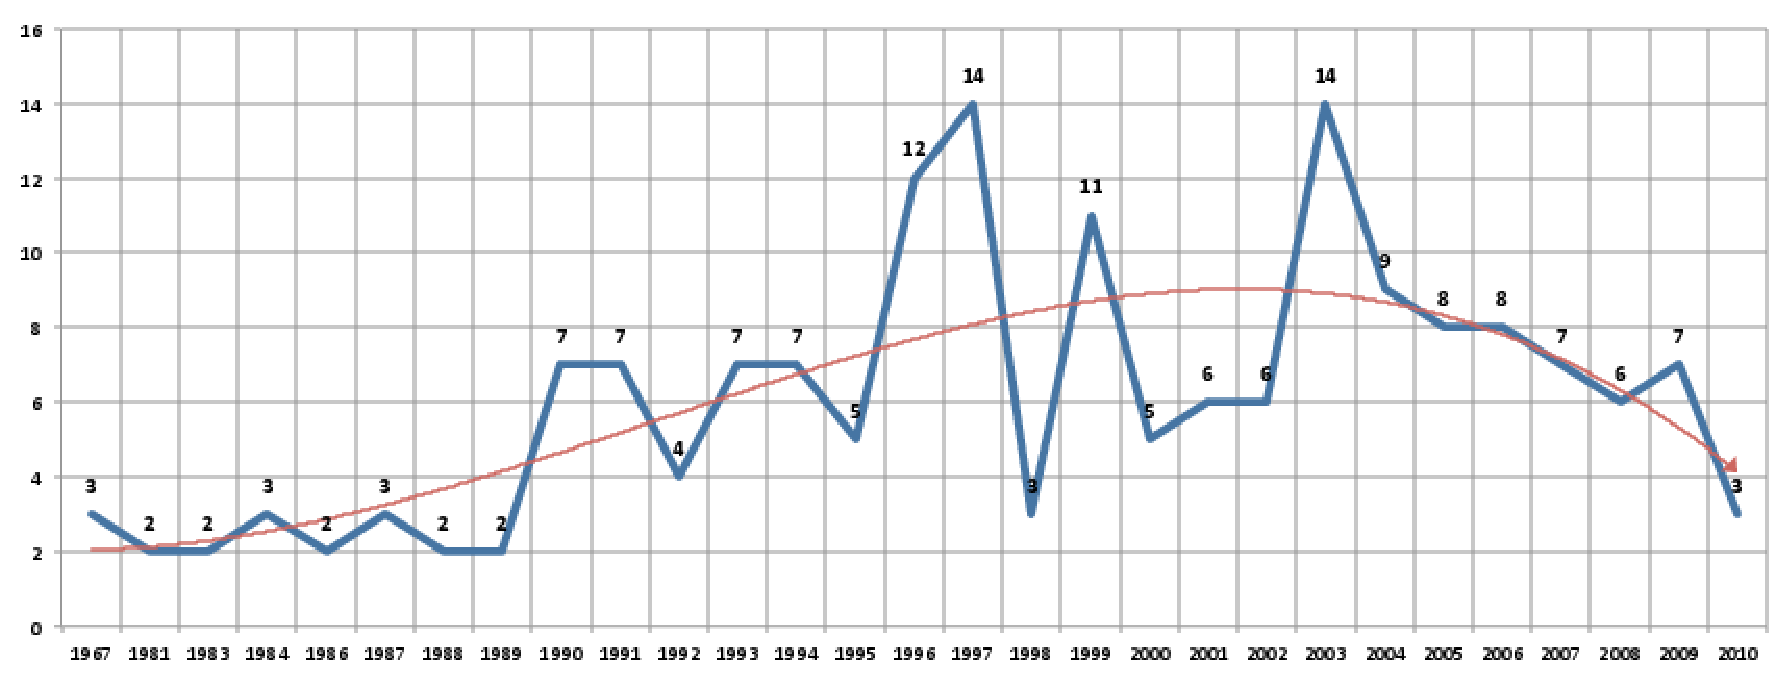
\includegraphics[scale=0.5]{conteudo/capitulos/figs/modelo-img-grafico.eps}
	\end{center}
	\legend{Fonte: \citeonline[p. 24]{araujo2012}}
\end{figure}

% ---
\subsection{Figuras em \emph{minipages}}
% ---

\emph{Minipages} são usadas para inserir textos ou outros elementos em quadros
com tamanhos e posições controladas. Veja o exemplo da
\autoref{fig_minipage_imagem1} e da \autoref{fig_minipage_grafico2}.

\begin{figure}[htb]
 \label{teste}
 \centering
  \begin{minipage}{0.4\textwidth}
    \centering
    \caption{Imagem 1 da minipage} \label{fig_minipage_imagem1}
    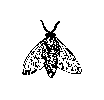
\includegraphics[scale=0.9]{conteudo/capitulos/figs/fly.eps}
    \legend{Fonte: Produzido pelos autores}
  \end{minipage}
  \hfill
  \begin{minipage}{0.4\textwidth}
    \centering
    \caption{Grafico 2 da minipage} \label{fig_minipage_grafico2}
    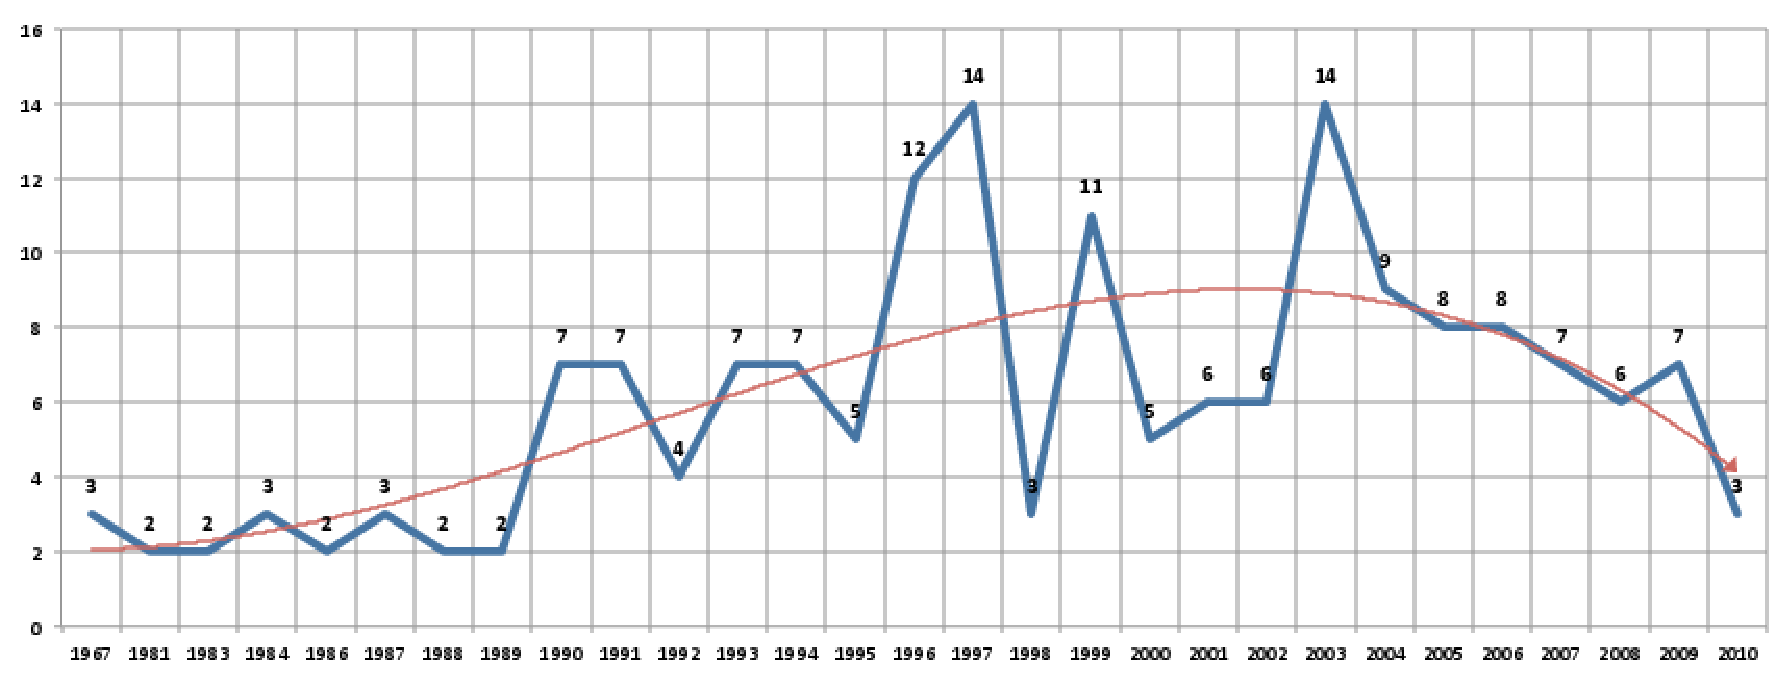
\includegraphics[scale=0.2]{conteudo/capitulos/figs/modelo-img-grafico.eps}
    \legend{Fonte: \citeonline[p. 24]{araujo2012}}
  \end{minipage}
\end{figure}

Observe que, segundo a \citeonline[seções 4.2.1.10 e 5.8]{NBR14724:2011}, as
ilustrações devem sempre ter numeração contínua e única em todo o documento:

\begin{citacao}
Qualquer que seja o tipo de ilustração, sua identificação aparece na parte
superior, precedida da palavra designativa (desenho, esquema, fluxograma,
fotografia, gráfico, mapa, organograma, planta, quadro, retrato, figura,
imagem, entre outros), seguida de seu número de ordem de ocorrência no texto,
em algarismos arábicos, travessão e do respectivo título. Após a ilustração, na
parte inferior, indicar a fonte consultada (elemento obrigatório, mesmo que
seja produção do próprio autor), legenda, notas e outras informações
necessárias à sua compreensão (se houver). A ilustração deve ser citada no
texto e inserida o mais próximo possível do trecho a que se
refere. \cite[seções 5.8]{NBR14724:2011}
\end{citacao}

% ---
\section{Expressões matemáticas}
% ---

\index{expressões matemáticas}Use o ambiente \texttt{equation} para escrever
expressões matemáticas numeradas:

\begin{equation}
  \forall x \in X, \quad \exists \: y \leq \epsilon
\end{equation}

Escreva expressões matemáticas entre \$ e \$, como em $ \lim_{x \to \infty}
\exp(-x) = 0 $, para que fiquem na mesma linha.

Também é possível usar colchetes para indicar o início de uma expressão
matemática que não é numerada.

\[
\left|\sum_{i=1}^n a_ib_i\right|
\le
\left(\sum_{i=1}^n a_i^2\right)^{1/2}
\left(\sum_{i=1}^n b_i^2\right)^{1/2}
\]

Consulte mais informações sobre expressões matemáticas em
\url{https://code.google.com/p/abntex2/wiki/Referencias}.

% ---
\section{Enumerações: alíneas e subalíneas}
% ---

\index{alíneas}\index{subalíneas}\index{incisos}Quando for necessário enumerar
os diversos assuntos de uma seção que não possua título, esta deve ser
subdividida em alíneas \cite[4.2]{NBR6024:2012}:

\begin{alineas}

  \item os diversos assuntos que não possuam título próprio, dentro de uma mesma
  seção, devem ser subdivididos em alíneas; 
  
  \item o texto que antecede as alíneas termina em dois pontos;
  \item as alíneas devem ser indicadas alfabeticamente, em letra minúscula,
  seguida de parêntese. Utilizam-se letras dobradas, quando esgotadas as
  letras do alfabeto;

  \item as letras indicativas das alíneas devem apresentar recuo em relação à
  margem esquerda;

  \item o texto da alínea deve começar por letra minúscula e terminar em
  ponto-e-vírgula, exceto a última alínea que termina em ponto final;

  \item o texto da alínea deve terminar em dois pontos, se houver subalínea;

  \item a segunda e as seguintes linhas do texto da alínea começa sob a
  primeira letra do texto da própria alínea;
  
  \item subalíneas \cite[4.3]{NBR6024:2012} devem ser conforme as alíneas a
  seguir:

  \begin{alineas}
     \item as subalíneas devem começar por travessão seguido de espaço;

     \item as subalíneas devem apresentar recuo em relação à alínea;

     \item o texto da subalínea deve começar por letra minúscula e terminar em
     ponto-e-vírgula. A última subalínea deve terminar em ponto final, se não
     houver alínea subsequente;

     \item a segunda e as seguintes linhas do texto da subalínea começam sob a
     primeira letra do texto da própria subalínea.
  \end{alineas}
  
  \item no \abnTeX\ estão disponíveis os ambientes \texttt{incisos} e
  \texttt{subalineas}, que em suma são o mesmo que se criar outro nível de
  \texttt{alineas}, como nos exemplos à seguir:
  
  \begin{incisos}
    \item \textit{Um novo inciso em itálico};
  \end{incisos}
  
  \item Alínea em \textbf{negrito}:
  
  \begin{subalineas}
    \item \textit{Uma subalínea em itálico};
    \item \underline{\textit{Uma subalínea em itálico e sublinhado}}; 
  \end{subalineas}
  
  \item Última alínea com \emph{ênfase}.
  
\end{alineas}

% ---
\section{Espaçamento entre parágrafos e linhas}
% ---

\index{espaçamento!dos parágrafos}O tamanho do parágrafo, espaço entre a margem
e o início da frase do parágrafo, é definido por:

\begin{verbatim}
   \setlength{\parindent}{1.3cm}
\end{verbatim}

\index{espaçamento!do primeiro parágrafo}Por padrão, não há espaçamento no
primeiro parágrafo de cada início de divisão do documento
(\autoref{sec-divisoes}). Porém, você pode definir que o primeiro parágrafo
também seja indentado, como é o caso deste documento. Para isso, apenas inclua o
pacote \textsf{indentfirst} no preâmbulo do documento:

\begin{verbatim}
   \usepackage{indentfirst}      % Indenta o primeiro parágrafo de cada seção.
\end{verbatim}

\index{espaçamento!entre os parágrafos}O espaçamento entre um parágrafo e outro
pode ser controlado por meio do comando:

\begin{verbatim}
  \setlength{\parskip}{0.2cm}  % tente também \onelineskip
\end{verbatim}

\index{espaçamento!entre as linhas}O controle do espaçamento entre linhas é
definido por:

\begin{verbatim}
  \OnehalfSpacing       % espaçamento um e meio (padrão); 
  \DoubleSpacing        % espaçamento duplo
  \SingleSpacing        % espaçamento simples	
\end{verbatim}

Para isso, também estão disponíveis os ambientes:

\begin{verbatim}
  \begin{SingleSpace} ...\end{SingleSpace}
  \begin{Spacing}{hfactori} ... \end{Spacing}
  \begin{OnehalfSpace} ... \end{OnehalfSpace}
  \begin{OnehalfSpace*} ... \end{OnehalfSpace*}
  \begin{DoubleSpace} ... \end{DoubleSpace}
  \begin{DoubleSpace*} ... \end{DoubleSpace*} 
\end{verbatim}

Para mais informações, consulte \citeonline[p. 47-52 e 135]{memoir}.

% ---
\section{Inclusão de outros arquivos}\label{sec-include}
% ---

É uma boa prática dividir o seu documento em diversos arquivos, e não
apenas escrever tudo em um único. Esse recurso foi utilizado neste
documento. Para incluir diferentes arquivos em um arquivo principal,
de modo que cada arquivo incluído fique em uma página diferente, utilize o
comando:

\begin{verbatim}
   \include{documento-a-ser-incluido}      % sem a extensão .tex
\end{verbatim}

Para incluir documentos sem quebra de páginas, utilize:

\begin{verbatim}
   \input{documento-a-ser-incluido}      % sem a extensão .tex
\end{verbatim}

% ---
\section{Compilar o documento \LaTeX}
% ---

Geralmente os editores \LaTeX, como o
TeXlipse\footnote{\url{http://texlipse.sourceforge.net/}}, o
Texmaker\footnote{\url{http://www.xm1math.net/texmaker/}}, entre outros,
compilam os documentos automaticamente, de modo que você não precisa se
preocupar com isso.

No entanto, você pode compilar os documentos \LaTeX usando os seguintes
comandos, que devem ser digitados no \emph{Prompt de Comandos} do Windows ou no
\emph{Terminal} do Mac ou do Linux:

\begin{verbatim}
   pdflatex ARQUIVO_PRINCIPAL.tex
   bibtex ARQUIVO_PRINCIPAL.aux
   makeindex ARQUIVO_PRINCIPAL.idx 
   makeindex ARQUIVO_PRINCIPAL.nlo -s nomencl.ist -o ARQUIVO_PRINCIPAL.nls
   pdflatex ARQUIVO_PRINCIPAL.tex
   pdflatex ARQUIVO_PRINCIPAL.tex
\end{verbatim}

% ---
\section{Remissões internas}
% ---

Ao nomear a \autoref{tab-nivinv} e a \autoref{fig_circulo}, apresentamos um
exemplo de remissão interna, que também pode ser feita quando indicamos o
\autoref{cap_exemplos}, que tem o nome \emph{\nameref{cap_exemplos}}. O número
do capítulo indicado é \ref{cap_exemplos}, que se inicia à
\autopageref{cap_exemplos}\footnote{O número da página de uma remissão pode ser
obtida também assim:
\pageref{cap_exemplos}.}.
Veja a \autoref{sec-divisoes} para outros exemplos de remissões internas entre
seções, subseções e subsubseções.

O código usado para produzir o texto desta seção é:

\begin{verbatim}
Ao nomear a \autoref{tab-nivinv} e a \autoref{fig_circulo}, apresentamos um
exemplo de remissão interna, que também pode ser feita quando indicamos o
\autoref{cap_exemplos}, que tem o nome \emph{\nameref{cap_exemplos}}. O número
do capítulo indicado é \ref{cap_exemplos}, que se inicia à
\autopageref{cap_exemplos}\footnote{O número da página de uma remissão pode ser
obtida também assim:
\pageref{cap_exemplos}.}.
Veja a \autoref{sec-divisoes} para outros exemplos de remissões internas entre
seções, subseções e subsubseções.
\end{verbatim}

% ---
\section{Divisões do documento: seção}\label{sec-divisoes}
% ---

Esta seção testa o uso de divisões de documentos. Esta é a
\autoref{sec-divisoes}. Veja a \autoref{sec-divisoes-subsection}.

\subsection{Divisões do documento: subseção}\label{sec-divisoes-subsection}

Isto é uma subseção. Veja a \autoref{sec-divisoes-subsubsection}, que é uma
\texttt{subsubsection} do \LaTeX, mas é impressa chamada de ``subseção'' porque
no Português não temos a palavra ``subsubseção''.

\subsubsection{Divisões do documento: subsubseção}
\label{sec-divisoes-subsubsection}

Isto é uma subsubseção.

\subsubsection{Divisões do documento: subsubseção}

Isto é outra subsubseção.

\subsection{Divisões do documento: subseção}\label{sec-exemplo-subsec}

Isto é uma subseção.

\subsubsection{Divisões do documento: subsubseção}

Isto é mais uma subsubseção da \autoref{sec-exemplo-subsec}.


\subsubsubsection{Esta é uma subseção de quinto
nível}\label{sec-exemplo-subsubsubsection}

Esta é uma seção de quinto nível. Ela é produzida com o seguinte comando:

\begin{verbatim}
\subsubsubsection{Esta é uma subseção de quinto
nível}\label{sec-exemplo-subsubsubsection}
\end{verbatim}

\subsubsubsection{Esta é outra subseção de quinto nível}\label{sec-exemplo-subsubsubsection-outro}

Esta é outra seção de quinto nível.


\paragraph{Este é um parágrafo numerado}\label{sec-exemplo-paragrafo}

Este é um exemplo de parágrafo nomeado. Ele é produzida com o comando de
parágrafo:

\begin{verbatim}
\paragraph{Este é um parágrafo nomeado}\label{sec-exemplo-paragrafo}
\end{verbatim}

A numeração entre parágrafos numerados e subsubsubseções são contínuas.

\paragraph{Esta é outro parágrafo numerado}\label{sec-exemplo-paragrafo-outro}

Esta é outro parágrafo nomeado.

% ---
\section{Outro exemplo de seção}
% ---

Isso atende à norma \citeonline[seções de 5.2.2 a 5.2.4]{NBR14724:2011} 
 e \citeonline[seções de 3.1 a 3.8]{NBR6024:2012}.

% ---
\section{Diferentes idiomas e hifenizações}
\label{sec-hifenizacao}
% ---

Para usar hifenizações de diferentes idiomas, inclua nas opções do documento o
nome dos idiomas que o seu texto contém. Por exemplo (para melhor
visualização, as opções foram quebras em diferentes linhas):

\begin{verbatim}
\documentclass[
	12pt,
	openright,
	twoside,
	a4paper,
	english,
	french,
	spanish,
	brazil
	]{abntex2}
\end{verbatim}

O idioma português-brasileiro (\texttt{brazil}) é incluído automaticamente pela
classe \textsf{abntex2}. Porém, mesmo assim a opção \texttt{brazil} deve ser
informada como a última opção da classe para que todos os pacotes reconheçam o
idioma. Vale ressaltar que a última opção de idioma é a utilizada por padrão no
documento. Desse modo, caso deseje escrever um texto em inglês que tenha
citações em português e em francês, você deveria usar o preâmbulo como abaixo:

\begin{verbatim}
\documentclass[
	12pt,
	openright,
	twoside,
	a4paper,
	french,
	brazil,
	english
	]{abntex2}
\end{verbatim}

A lista completa de idiomas suportados, bem como outras opções de hifenização,
estão disponíveis em \citeonline[p.~5-6]{babel}.

Exemplo de hifenização em inglês\footnote{Extraído de:
\url{http://en.wikibooks.org/wiki/LaTeX/Internationalization}}:

\begin{otherlanguage*}{english}
\textit{Text in English language. This environment switches all language-related
definitions, like the language specific names for figures, tables etc. to the other
language. The starred version of this environment typesets the main text
according to the rules of the other language, but keeps the language specific
string for ancillary things like figures, in the main language of the document.
The environment hyphenrules switches only the hyphenation patterns used; it can
also be used to disallow hyphenation by using the language name
`nohyphenation'.}
\end{otherlanguage*}

O idioma geral do texto por ser alterado como no exemplo seguinte:

\begin{verbatim}
  \selectlanguage{english}
\end{verbatim}

Isso altera automaticamente a hifenização e todos os nomes constantes de
referências do documento para o idioma inglês. Consulte o manual da classe
\cite{abntex2classe} para obter orientações adicionais sobre internacionalização de
documentos produzidos com \abnTeX.

A \autoref{sec-citacao} descreve o ambiente \texttt{citacao} que pode receber
como parâmetro um idioma a ser usado na citação.

% ---
\section{Consulte o manual da classe \textsf{abntex2}}
% ---

Consulte o manual da classe \textsf{abntex2} \cite{abntex2classe} para uma
referência completa das macros e ambientes disponíveis. 

Além disso, o manual possui informações adicionais sobre as normas ABNT
observadas pelo \abnTeX\ e considerações sobre eventuais requisitos específicos
não atendidos, como o caso da \citeonline[seção 5.2.2]{NBR14724:2011}, que
especifica o espaçamento entre os capítulos e o início do texto, regra
propositalmente não atendida pelo presente modelo \cite{masolo2010}.

% ---
\section{Referências bibliográficas}
% ---

A formatação das referências bibliográficas conforme as regras da ABNT são um
dos principais objetivos do \abnTeX. Consulte os manuais
\citeonline{abntex2cite} e \citeonline{abntex2cite-alf} para obter informações
sobre como utilizar as referências bibliográficas.

%-
\subsection{Acentuação de referências bibliográficas}
%-

Normalmente não há problemas em usar caracteres acentuados em arquivos
bibliográficos (\texttt{*.bib}). Porém, como as regras da ABNT fazem uso quase
abusivo da conversão para letras maiúsculas, é preciso observar o modo como se
escreve os nomes dos autores. Na ~\autoref{tabela-acentos} você encontra alguns
exemplos das conversões mais importantes. Preste atenção especial para `ç' e `í'
que devem estar envoltos em chaves. A regra geral é sempre usar a acentuação
neste modo quando houver conversão para letras maiúsculas.

\begin{table}[htbp]
\caption{Tabela de conversão de acentuação.}
\label{tabela-acentos}

\begin{center}
\begin{tabular}{ll}\hline\hline
acento & \textsf{bibtex}\\
à á ã & \verb+\`a+ \verb+\'a+ \verb+\~a+\\
í & \verb+{\'\i}+\\
ç & \verb+{\c c}+\\
\hline\hline
\end{tabular}
\end{center}
\end{table}


% ---
\section{Precisa de ajuda?}
% ---

Consulte a FAQ com perguntas frequentes e comuns no portal do \abnTeX:
\url{https://code.google.com/p/abntex2/wiki/FAQ}.

Inscreva-se no grupo de usuários \LaTeX:
\url{http://groups.google.com/group/latex-br}, tire suas dúvidas e ajude
outros usuários.

Participe também do grupo de desenvolvedores do \abnTeX:
\url{http://groups.google.com/group/abntex2} e faça sua contribuição à
ferramenta.
